\documentclass[]{tufte-handout}

% ams
\usepackage{amssymb,amsmath}

\usepackage{ifxetex,ifluatex}
\usepackage{fixltx2e} % provides \textsubscript
\ifnum 0\ifxetex 1\fi\ifluatex 1\fi=0 % if pdftex
  \usepackage[T1]{fontenc}
  \usepackage[utf8]{inputenc}
\else % if luatex or xelatex
  \makeatletter
  \@ifpackageloaded{fontspec}{}{\usepackage{fontspec}}
  \makeatother
  \defaultfontfeatures{Ligatures=TeX,Scale=MatchLowercase}
  \makeatletter
  \@ifpackageloaded{soul}{
     \renewcommand\allcapsspacing[1]{{\addfontfeature{LetterSpace=15}#1}}
     \renewcommand\smallcapsspacing[1]{{\addfontfeature{LetterSpace=10}#1}}
   }{}
  \makeatother

\fi

% graphix
\usepackage{graphicx}
\setkeys{Gin}{width=\linewidth,totalheight=\textheight,keepaspectratio}

% booktabs
\usepackage{booktabs}

% url
\usepackage{url}

% hyperref
\usepackage{hyperref}

% units.
\usepackage{units}


\setcounter{secnumdepth}{-1}

% citations
\usepackage{natbib}
\bibliographystyle{plainnat}


% pandoc syntax highlighting
\usepackage{color}
\usepackage{fancyvrb}
\newcommand{\VerbBar}{|}
\newcommand{\VERB}{\Verb[commandchars=\\\{\}]}
\DefineVerbatimEnvironment{Highlighting}{Verbatim}{commandchars=\\\{\}}
% Add ',fontsize=\small' for more characters per line
\newenvironment{Shaded}{}{}
\newcommand{\AlertTok}[1]{\textcolor[rgb]{1.00,0.00,0.00}{\textbf{#1}}}
\newcommand{\AnnotationTok}[1]{\textcolor[rgb]{0.38,0.63,0.69}{\textbf{\textit{#1}}}}
\newcommand{\AttributeTok}[1]{\textcolor[rgb]{0.49,0.56,0.16}{#1}}
\newcommand{\BaseNTok}[1]{\textcolor[rgb]{0.25,0.63,0.44}{#1}}
\newcommand{\BuiltInTok}[1]{#1}
\newcommand{\CharTok}[1]{\textcolor[rgb]{0.25,0.44,0.63}{#1}}
\newcommand{\CommentTok}[1]{\textcolor[rgb]{0.38,0.63,0.69}{\textit{#1}}}
\newcommand{\CommentVarTok}[1]{\textcolor[rgb]{0.38,0.63,0.69}{\textbf{\textit{#1}}}}
\newcommand{\ConstantTok}[1]{\textcolor[rgb]{0.53,0.00,0.00}{#1}}
\newcommand{\ControlFlowTok}[1]{\textcolor[rgb]{0.00,0.44,0.13}{\textbf{#1}}}
\newcommand{\DataTypeTok}[1]{\textcolor[rgb]{0.56,0.13,0.00}{#1}}
\newcommand{\DecValTok}[1]{\textcolor[rgb]{0.25,0.63,0.44}{#1}}
\newcommand{\DocumentationTok}[1]{\textcolor[rgb]{0.73,0.13,0.13}{\textit{#1}}}
\newcommand{\ErrorTok}[1]{\textcolor[rgb]{1.00,0.00,0.00}{\textbf{#1}}}
\newcommand{\ExtensionTok}[1]{#1}
\newcommand{\FloatTok}[1]{\textcolor[rgb]{0.25,0.63,0.44}{#1}}
\newcommand{\FunctionTok}[1]{\textcolor[rgb]{0.02,0.16,0.49}{#1}}
\newcommand{\ImportTok}[1]{#1}
\newcommand{\InformationTok}[1]{\textcolor[rgb]{0.38,0.63,0.69}{\textbf{\textit{#1}}}}
\newcommand{\KeywordTok}[1]{\textcolor[rgb]{0.00,0.44,0.13}{\textbf{#1}}}
\newcommand{\NormalTok}[1]{#1}
\newcommand{\OperatorTok}[1]{\textcolor[rgb]{0.40,0.40,0.40}{#1}}
\newcommand{\OtherTok}[1]{\textcolor[rgb]{0.00,0.44,0.13}{#1}}
\newcommand{\PreprocessorTok}[1]{\textcolor[rgb]{0.74,0.48,0.00}{#1}}
\newcommand{\RegionMarkerTok}[1]{#1}
\newcommand{\SpecialCharTok}[1]{\textcolor[rgb]{0.25,0.44,0.63}{#1}}
\newcommand{\SpecialStringTok}[1]{\textcolor[rgb]{0.73,0.40,0.53}{#1}}
\newcommand{\StringTok}[1]{\textcolor[rgb]{0.25,0.44,0.63}{#1}}
\newcommand{\VariableTok}[1]{\textcolor[rgb]{0.10,0.09,0.49}{#1}}
\newcommand{\VerbatimStringTok}[1]{\textcolor[rgb]{0.25,0.44,0.63}{#1}}
\newcommand{\WarningTok}[1]{\textcolor[rgb]{0.38,0.63,0.69}{\textbf{\textit{#1}}}}

% longtable
\usepackage{longtable,booktabs}

% multiplecol
\usepackage{multicol}

% strikeout
\usepackage[normalem]{ulem}

% morefloats
\usepackage{morefloats}


% tightlist macro required by pandoc >= 1.14
\providecommand{\tightlist}{%
  \setlength{\itemsep}{0pt}\setlength{\parskip}{0pt}}

% title / author / date
\title[正規分布表を求めるには]{正規分布表を求めるには}
\author{Sampo Suzuki, CC 4.0 BY-NC-SA}
\date{2021-06-04}

% --- 参考資料 ----------------------------------------------------------------
% https://github.com/Gedevan-Aleksizde/Japan.R2019/blob/master/latex/preamble.tex
% https://teastat.blogspot.com/2019/01/bookdown.html

% --- Packages ----------------------------------------------------------------
% 日本語とtufte, kableExtraを使うために必要なTeXパッケージ指定
% tufteではA4サイズの指定が不可能
%  A4 210mm x 297mm
%   \usepackage[a4paper, total={6.5in, 9.5in}]{geometry}
%   \usepackage{indentfirst}   # tinytexのリポジトリには存在しない?
% \usepackage[a4paper, total={160mm, 247mm}, left=25mm, top=25mm]{geometry}
% \usepackage[pdfbox,tombo]{gentombow}  % トンボを設定する場合は有効にする
\usepackage{ifthen}                     % 条件分岐用 \ifthenelse{条件}{T}{F}
\usepackage{booktabs}                   % ここからkableExtra用パッケージ
\usepackage{longtable}                  % 
\usepackage{array}                      % 
\usepackage{multirow}                   % 
\usepackage{wrapfig}                    % 
\usepackage{float}                      % 
\usepackage{colortbl}                   % 
\usepackage{pdflscape}                  % 
\usepackage{tabu}                       % 
\usepackage{threeparttable}             % 
\usepackage{threeparttablex}            % 
\usepackage[normalem]{ulem}             % 
\usepackage{inputenc}                   % 
\usepackage{makecell}                   % 
\usepackage{xcolor}                     % ここまでkableExtra用
\usepackage{amsmath}                    % 
\usepackage{fontawesome5}               % fontawesomeを使うために必要
\usepackage{subfig}                     % 複数の図を並べる際に必要(古い?)
% \usepackage{subcaption}                 % 同上(新しい?)
\usepackage{xeCJK}                      % 以下、日本語フォント用に必要
\usepackage[noto]{zxjafont}             % Linux環境ではこちを指定
% \usepackage[haranoaji]{zxjafont}      % Windows環境ではこちらを指定する
\usepackage{zxjatype}                   % 日本語処理に必要
\usepackage{pxrubrica}                  % ルビ用
\usepackage{hyperref}                   % ハイパーリンク用必要?

% --- Index ------------------------------------------------------------------
% https://texwiki.texjp.org/?%E7%B4%A2%E5%BC%95%E4%BD%9C%E6%88%90
% これを指定するとIndex(索引)は作成されるが参照ページがズレる
% 中間ファイルの.indではページはズレていないので、その後の結合処理がおかしい
% \usepackage{makeidx}
% \makeindex
% \usepackage{showidx}                  % 索引確認用

% --- Table of Contentes ------------------------------------------------------
% TOCにLOT(List of Tables), LOF(List of Figures), Bibliography, Indexを表示
% \usepackage[nottoc]{tocbibind}

% --- Fonts -------------------------------------------------------------------
% フォントしては index.html でも可能(pandoc用オプションは index.htmlにて)
% \setCJKmonofont{Source Han Code JP}
\setmonofont{Source Han Code JP}     % Linuxではこれのみコメントアウトする
% \setjamonofont{Source Han Code JP}

% ## 日本語フォントの扱いについてはzxjafontパッケージの解説を参照のこと
% # https://mirror.las.iastate.edu/tex-archive/language/japanese/zxjafont/zxjafont.pdf
% #
% ## Windows環境ではなぜかNotoフォントが認識されないので源ノシリーズベースの
% ## 原ノ味フォントかIPAexフォントを利用する(原ノ味はtlmgrでインストール可)
% # \usepackage[haranoaji]{zxjafont}
% # \usepackage[ipaex]{zxjafont}
% #
% ## Windows環境でNotoフォントを指定したい場合は以下のようにheader-includeで
% ## 個別に指定する(setCJKxxxfotnの指定は必要?)
% # \setmainfont{NotoSerifCJKjp-Regular.otf}[BoldFont=NotoSerifCJKjp-Bold.otf]
% # \setsansfont{NotoSansCJKjp-Regular.otf}[BoldFont=NotoSansCJKjp-Bold.otf]
% # \setmonofont{NotoSansMonoCJKjp-Regular.otf}[BoldFont=NotoSansMonoCJKjp-Bold.otf]
% ## モノフォントは源ノ角コード(Source Code Proの日本語版)がおすゝめ
% # \setmonofont{SourceHanCodeJP-Regular.otf}[BoldFont=SourceHanCodeJPS-Bold.otf]

\begin{document}

\maketitle




\hypertarget{introduction}{%
\section{\texorpdfstring{\textbf{Introduction}}{Introduction}}\label{introduction}}

 正規分布表は\(0\)から任意の\(Z\)スコアまでに含まれる正規分布の面積を求める表です。逆引きすることで、面積から\(Z\)スコアを求めることもできます。例えば\(95\%\)の面積になる\(Z\)スコアは正規分布表から片側面積の\(47.5\%\)に最も近い値を探すと\(Z = 1.96\)になります。

\begin{marginfigure}

{\centering 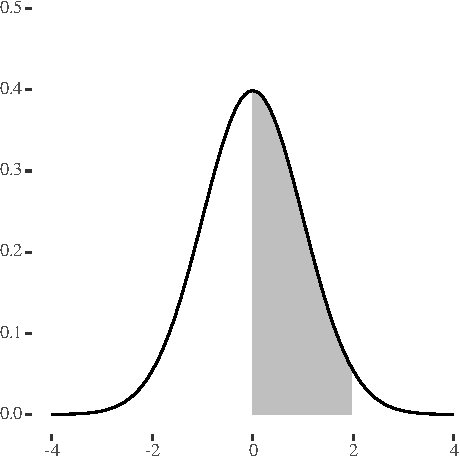
\includegraphics{NormTable_files/figure-latex/unnamed-chunk-1-1} 

}

\caption[正規分布表で求められる面積]{正規分布表で求められる面積}\label{fig:unnamed-chunk-1}
\end{marginfigure}

 

\hypertarget{rux3067ux6c42ux3081ux308b}{%
\section{\texorpdfstring{\textbf{Rで求める}}{Rで求める}}\label{rux3067ux6c42ux3081ux308b}}

 \textbf{R}で\(Z\)スコアから正規分布の面積を求める場合は\texttt{pnorm()}関数、面積から\(Z\)スコアを求めるには\texttt{qnorm()}関数がありますが、引数の指定には注意が必要です。例えば両側面積が\(95\%\)になる\(Z\)スコアを求めようとして、以下のように指定してしまうと

\begin{Shaded}
\begin{Highlighting}[numbers=left,,]
\FunctionTok{qnorm}\NormalTok{(}\FloatTok{0.95}\NormalTok{)}
\end{Highlighting}
\end{Shaded}

\begin{verbatim}
## [1] 1.644854
\end{verbatim}

求められた\(Z\)スコアは明らかに正規分布表から得られる値とは異なっています。これは、\texttt{qnorm()}関数が下側(\texttt{-Inf})からの面積が\(95\%\)になる\(Z\)スコアを計算しているためです。図のように上側が\(5\%\)空いているわけですから、正規分布表では両側面積で\(90\%\)に相当する\(Z\)スコアを求めているためです。

\begin{marginfigure}

{\centering 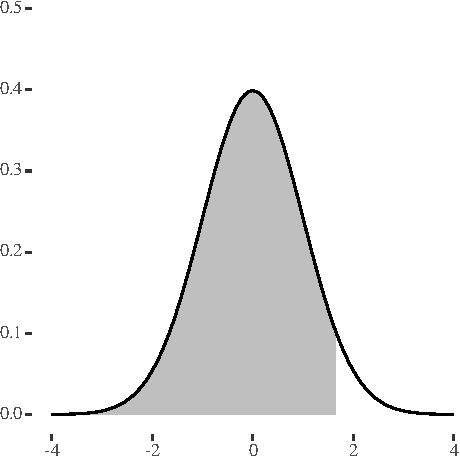
\includegraphics{NormTable_files/figure-latex/unnamed-chunk-3-1} 

}

\caption[`qnorm()`関数が求めている面積]{`qnorm()`関数が求めている面積}\label{fig:unnamed-chunk-3}
\end{marginfigure}

 \\
正規分布の確率密度関数(\texttt{dnorm()})を用いて下側(\texttt{-Inf})から求められた1.6448536まで積分すると値が一致していることがわかります。

\begin{Shaded}
\begin{Highlighting}[numbers=left,,]
\FunctionTok{integrate}\NormalTok{(dnorm, }\SpecialCharTok{{-}}\ConstantTok{Inf}\NormalTok{, }\FloatTok{1.644854}\NormalTok{)}
\end{Highlighting}
\end{Shaded}

\begin{verbatim}
## 0.95 with absolute error < 8.6e-08
\end{verbatim}

\(\pm1.6448536\)の範囲を積分すると正規分布表の値を倍にした値とほぼ一致していることもわかります。

\begin{Shaded}
\begin{Highlighting}[numbers=left,,]
\FunctionTok{integrate}\NormalTok{(dnorm, }\SpecialCharTok{{-}}\FloatTok{1.644854}\NormalTok{, }\FloatTok{1.644854}\NormalTok{)}
\end{Highlighting}
\end{Shaded}

\begin{verbatim}
## 0.9000001 with absolute error < 7.4e-14
\end{verbatim}

\newpage

\texttt{qnorm()}関数で正規分布表と同じ計算を行うためには両側で\(95\%\)、つまり、片側面積が\(\frac{1 - 0.95}{2} = 0.025\)となる上側(\texttt{Inf})から\(Z\)スコアを求める必要があります。

\begin{marginfigure}

{\centering 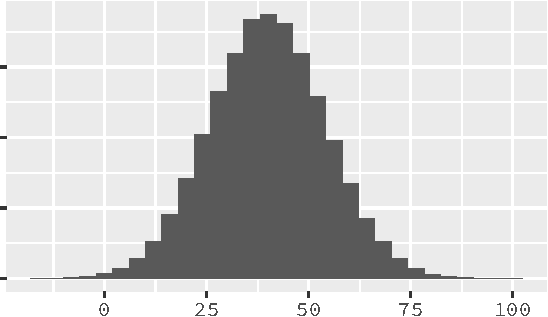
\includegraphics{NormTable_files/figure-latex/unnamed-chunk-6-1} 

}

\caption[上側$2.5\%$の面積を指定した場合]{上側$2.5\%$の面積を指定した場合}\label{fig:unnamed-chunk-6}
\end{marginfigure}

\begin{Shaded}
\begin{Highlighting}[numbers=left,,]
\FunctionTok{qnorm}\NormalTok{((}\DecValTok{1} \SpecialCharTok{{-}} \FloatTok{0.95}\NormalTok{) }\SpecialCharTok{/} \DecValTok{2}\NormalTok{, }\AttributeTok{lower.tail =} \ConstantTok{FALSE}\NormalTok{)}
\end{Highlighting}
\end{Shaded}

\begin{verbatim}
## [1] 1.959964
\end{verbatim}

同様に\(90\%\)であれば

\begin{marginfigure}

{\centering 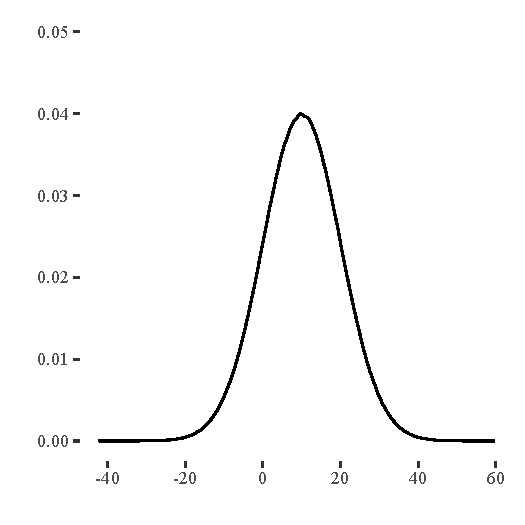
\includegraphics{NormTable_files/figure-latex/unnamed-chunk-8-1} 

}

\caption[上側$5\%$の面積を指定した場合]{上側$5\%$の面積を指定した場合}\label{fig:unnamed-chunk-8}
\end{marginfigure}

\begin{Shaded}
\begin{Highlighting}[numbers=left,,]
\FunctionTok{qnorm}\NormalTok{((}\DecValTok{1} \SpecialCharTok{{-}} \FloatTok{0.90}\NormalTok{) }\SpecialCharTok{/} \DecValTok{2}\NormalTok{, }\AttributeTok{lower.tail =} \ConstantTok{FALSE}\NormalTok{)}
\end{Highlighting}
\end{Shaded}

\begin{verbatim}
## [1] 1.644854
\end{verbatim}

\(68.3\%\)であれば

\begin{marginfigure}

{\centering \includegraphics{NormTable_files/figure-latex/unnamed-chunk-10-1} 

}

\caption[上側$15.85\%$の面積を指定した場合]{上側$15.85\%$の面積を指定した場合}\label{fig:unnamed-chunk-10}
\end{marginfigure}

\begin{Shaded}
\begin{Highlighting}[numbers=left,,]
\FunctionTok{qnorm}\NormalTok{((}\DecValTok{1} \SpecialCharTok{{-}} \FloatTok{0.683}\NormalTok{) }\SpecialCharTok{/} \DecValTok{2}\NormalTok{, }\AttributeTok{lower.tail =} \ConstantTok{FALSE}\NormalTok{)}
\end{Highlighting}
\end{Shaded}

\begin{verbatim}
## [1] 1.000642
\end{verbatim}

となります。

 

一方、\texttt{pnorm()}関数は\(Z\)スコアから正規分布の面積を求める関数で\texttt{qnorm()}と同様の考え方で計算しますので、\(Z\)スコアが\(1.0, 1.65, 1.96\)の場合、その上側の片側面積は

\begin{Shaded}
\begin{Highlighting}[numbers=left,,]
\FunctionTok{pnorm}\NormalTok{(}\FunctionTok{c}\NormalTok{(}\FloatTok{1.00}\NormalTok{, }\FloatTok{1.65}\NormalTok{, }\FloatTok{1.96}\NormalTok{), }\AttributeTok{lower.tail =} \ConstantTok{FALSE}\NormalTok{)}
\end{Highlighting}
\end{Shaded}

\begin{verbatim}
## [1] 0.15865525 0.04947147 0.02499790
\end{verbatim}

となります。両側面積は片側の\(50\%\)から上記を引いたものを倍にすれば良いことがわかります。

\begin{Shaded}
\begin{Highlighting}[numbers=left,,]
\NormalTok{(}\FunctionTok{pnorm}\NormalTok{(}\DecValTok{0}\NormalTok{) }\SpecialCharTok{{-}} \FunctionTok{pnorm}\NormalTok{(}\FunctionTok{c}\NormalTok{(}\FloatTok{1.00}\NormalTok{, }\FloatTok{1.65}\NormalTok{, }\FloatTok{1.96}\NormalTok{), }\AttributeTok{lower.tail =} \ConstantTok{FALSE}\NormalTok{)) }\SpecialCharTok{*} \DecValTok{2}
\end{Highlighting}
\end{Shaded}

\begin{verbatim}
## [1] 0.6826895 0.9010571 0.9500042
\end{verbatim}

 

\hypertarget{ux307eux3068ux3081}{%
\section{まとめ}\label{ux307eux3068ux3081}}

 \texttt{qnorm()}関数を用いる場合は正規分布表とは逆に上限(\texttt{Inf})側からの値を指定、\texttt{pnorm()}関数を用いる場合は求められた値を\(0.5\)から引いたものを\(2\)倍することで、正規分布表と同等の値を得ることができます。

\newpage

\hypertarget{ux554fux984c}{%
\subsection{問題}\label{ux554fux984c}}

 \texttt{pnorm()}関数を用いて正規分布表を作成しなさい。

\begin{longtable}[]{@{}lrrrrrrrrrr@{}}
\toprule
& X0.00 & X0.01 & X0.02 & X0.03 & X0.04 & X0.05 & X0.06 & X0.07 & X0.08
& X0.09 \\
\midrule
\endhead
0 & 0.0000 & 0.0040 & 0.0080 & 0.0120 & 0.0160 & 0.0199 & 0.0239 &
0.0279 & 0.0319 & 0.0359 \\
0.1 & 0.0398 & 0.0438 & 0.0478 & 0.0517 & 0.0557 & 0.0596 & 0.0636 &
0.0675 & 0.0714 & 0.0753 \\
0.2 & 0.0793 & 0.0832 & 0.0871 & 0.0910 & 0.0948 & 0.0987 & 0.1026 &
0.1064 & 0.1103 & 0.1141 \\
0.3 & 0.1179 & 0.1217 & 0.1255 & 0.1293 & 0.1331 & 0.1368 & 0.1406 &
0.1443 & 0.1480 & 0.1517 \\
0.4 & 0.1554 & 0.1591 & 0.1628 & 0.1664 & 0.1700 & 0.1736 & 0.1772 &
0.1808 & 0.1844 & 0.1879 \\
0.5 & 0.1915 & 0.1950 & 0.1985 & 0.2019 & 0.2054 & 0.2088 & 0.2123 &
0.2157 & 0.2190 & 0.2224 \\
0.6 & 0.2257 & 0.2291 & 0.2324 & 0.2357 & 0.2389 & 0.2422 & 0.2454 &
0.2486 & 0.2517 & 0.2549 \\
0.7 & 0.2580 & 0.2611 & 0.2642 & 0.2673 & 0.2704 & 0.2734 & 0.2764 &
0.2794 & 0.2823 & 0.2852 \\
0.8 & 0.2881 & 0.2910 & 0.2939 & 0.2967 & 0.2995 & 0.3023 & 0.3051 &
0.3078 & 0.3106 & 0.3133 \\
0.9 & 0.3159 & 0.3186 & 0.3212 & 0.3238 & 0.3264 & 0.3289 & 0.3315 &
0.3340 & 0.3365 & 0.3389 \\
1 & 0.3413 & 0.3438 & 0.3461 & 0.3485 & 0.3508 & 0.3531 & 0.3554 &
0.3577 & 0.3599 & 0.3621 \\
1.1 & 0.3643 & 0.3665 & 0.3686 & 0.3708 & 0.3729 & 0.3749 & 0.3770 &
0.3790 & 0.3810 & 0.3830 \\
1.2 & 0.3849 & 0.3869 & 0.3888 & 0.3907 & 0.3925 & 0.3944 & 0.3962 &
0.3980 & 0.3997 & 0.4015 \\
1.3 & 0.4032 & 0.4049 & 0.4066 & 0.4082 & 0.4099 & 0.4115 & 0.4131 &
0.4147 & 0.4162 & 0.4177 \\
1.4 & 0.4192 & 0.4207 & 0.4222 & 0.4236 & 0.4251 & 0.4265 & 0.4279 &
0.4292 & 0.4306 & 0.4319 \\
1.5 & 0.4332 & 0.4345 & 0.4357 & 0.4370 & 0.4382 & 0.4394 & 0.4406 &
0.4418 & 0.4429 & 0.4441 \\
1.6 & 0.4452 & 0.4463 & 0.4474 & 0.4484 & 0.4495 & 0.4505 & 0.4515 &
0.4525 & 0.4535 & 0.4545 \\
1.7 & 0.4554 & 0.4564 & 0.4573 & 0.4582 & 0.4591 & 0.4599 & 0.4608 &
0.4616 & 0.4625 & 0.4633 \\
1.8 & 0.4641 & 0.4649 & 0.4656 & 0.4664 & 0.4671 & 0.4678 & 0.4686 &
0.4693 & 0.4699 & 0.4706 \\
1.9 & 0.4713 & 0.4719 & 0.4726 & 0.4732 & 0.4738 & 0.4744 & 0.4750 &
0.4756 & 0.4761 & 0.4767 \\
2 & 0.4772 & 0.4778 & 0.4783 & 0.4788 & 0.4793 & 0.4798 & 0.4803 &
0.4808 & 0.4812 & 0.4817 \\
2.1 & 0.4821 & 0.4826 & 0.4830 & 0.4834 & 0.4838 & 0.4842 & 0.4846 &
0.4850 & 0.4854 & 0.4857 \\
2.2 & 0.4861 & 0.4864 & 0.4868 & 0.4871 & 0.4875 & 0.4878 & 0.4881 &
0.4884 & 0.4887 & 0.4890 \\
2.3 & 0.4893 & 0.4896 & 0.4898 & 0.4901 & 0.4904 & 0.4906 & 0.4909 &
0.4911 & 0.4913 & 0.4916 \\
2.4 & 0.4918 & 0.4920 & 0.4922 & 0.4925 & 0.4927 & 0.4929 & 0.4931 &
0.4932 & 0.4934 & 0.4936 \\
2.5 & 0.4938 & 0.4940 & 0.4941 & 0.4943 & 0.4945 & 0.4946 & 0.4948 &
0.4949 & 0.4951 & 0.4952 \\
2.6 & 0.4953 & 0.4955 & 0.4956 & 0.4957 & 0.4959 & 0.4960 & 0.4961 &
0.4962 & 0.4963 & 0.4964 \\
2.7 & 0.4965 & 0.4966 & 0.4967 & 0.4968 & 0.4969 & 0.4970 & 0.4971 &
0.4972 & 0.4973 & 0.4974 \\
2.8 & 0.4974 & 0.4975 & 0.4976 & 0.4977 & 0.4977 & 0.4978 & 0.4979 &
0.4979 & 0.4980 & 0.4981 \\
2.9 & 0.4981 & 0.4982 & 0.4982 & 0.4983 & 0.4984 & 0.4984 & 0.4985 &
0.4985 & 0.4986 & 0.4986 \\
3 & 0.4987 & 0.4987 & 0.4987 & 0.4988 & 0.4988 & 0.4989 & 0.4989 &
0.4989 & 0.4990 & 0.4990 \\
\bottomrule
\end{longtable}

 

 

enjoy!

\bibliography{bib/references.bib}



\end{document}
